\level{1}{Casi d'uso}
L’analisi del capitolato, l’incontro con il proponente e la discussione tra gli \insrole{Analisti} hanno portato all'individuazione dei casi d'uso riportati di seguito. 
I casi d'uso sono suddivisi in tre categorie, in quanto il progetto prevede la creazione di tre sistemi differenti:
\begin{description}
	\item[Norris] sono i casi d'uso inerenti alle funzionalità offerte dal framework;
	\item[Applicazione Android] sono i casi d'uso inerenti all'utilizzo dell'applicazione Android;
	\item[Dashboard] sono i casi d'uso inerenti all'utilizzo della dashboard.
\end{description}
Ogni caso d'uso è identificato da un codice univoco. La descrizione del modo in cui un caso d'uso viene identificato  è rintracciabile nel documento \insdoc{Norme di Progetto v1.00}.


\level{2}{Norris}
	\level{3}{Relazione tra utenti e attori}
	\begin{figure}[H]
		\centering
		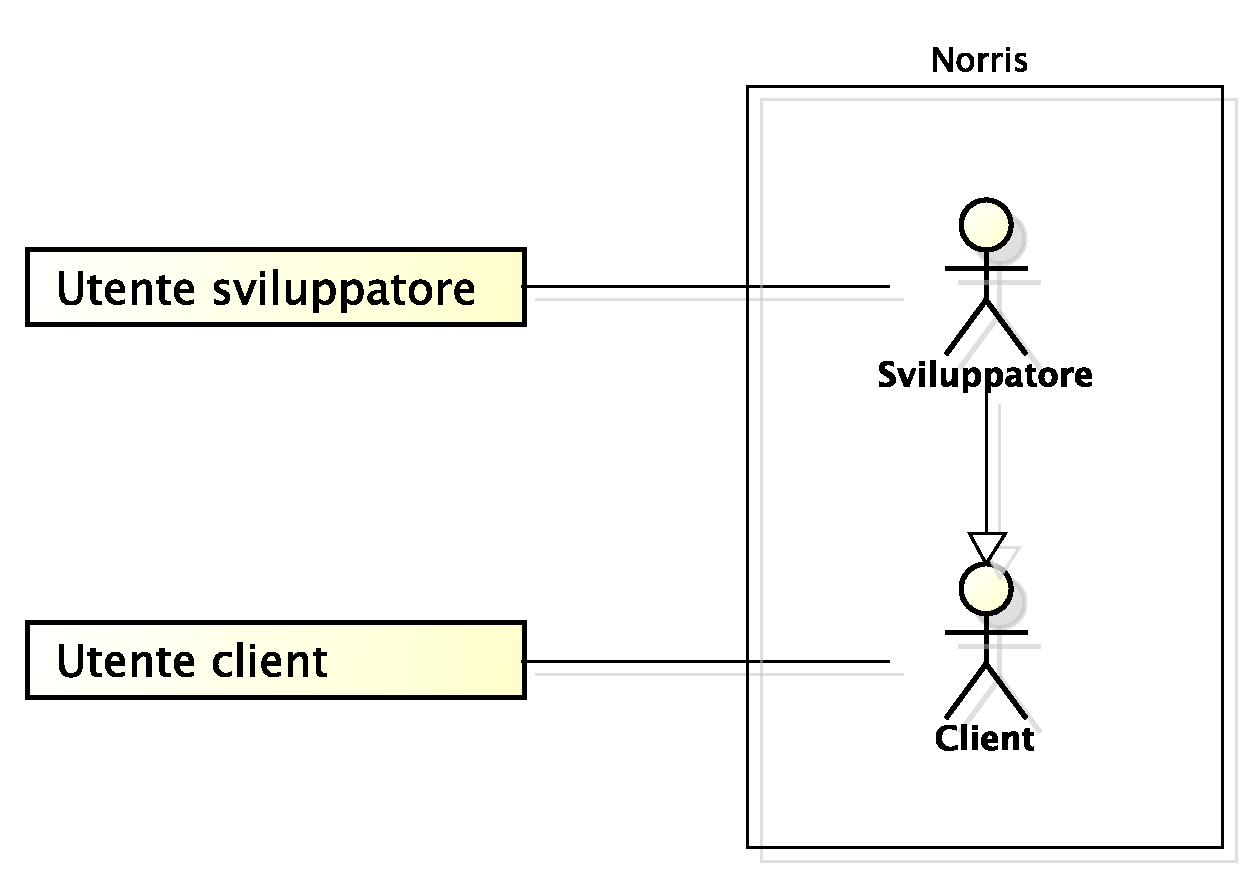
\includegraphics[scale=0.4]{Pics/UtentiAttoriNorris}
		\caption{Norris - Relazione tra utenti e attori}
	\end{figure}
	\input{UseCase/UCN.tex}

\level{2}{Applicazione Android}
	\level{3}{Relazione tra utenti e attori}
	\begin{figure}[H]
		\centering
		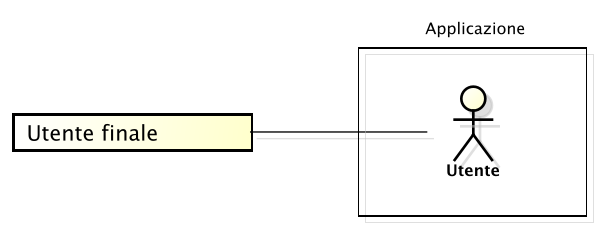
\includegraphics[scale=0.4]{Pics/UtentiAttoriApplicazione}
		\caption{Applicazione - Relazione tra utenti e attori}
	\end{figure}
	\input{UseCase/UCA.tex}

\level{2}{Dashboard}
	\level{3}{Relazione tra utenti e attori}
	\begin{figure}[H]
		\centering
		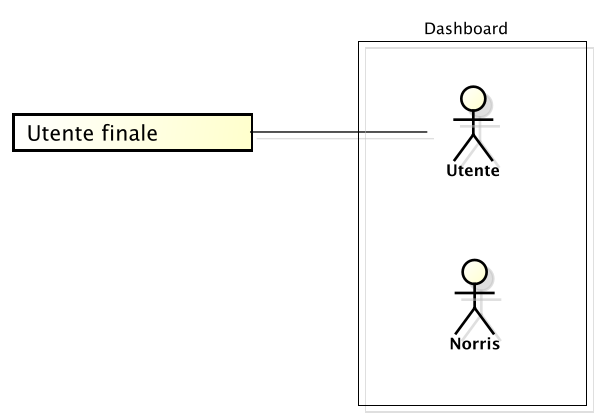
\includegraphics[scale=0.4]{Pics/UtentiAttoriDashboard}
		\caption{Dashboard - Relazione tra utenti e attori}
	\end{figure}
	\input{UseCase/UCD.tex}
